
% \begin{frame}
% \frametitle{Summary of Results}
% \vspace{2mm} 

% \end{frame}  

\begin{frame}
\frametitle{Scaling Laws and Small-scale Proxies} 
% \vspace{2.5mm}

\parbox{0.52\linewidth}{ 

\begin{minipage}[t]{1\linewidth} 
\begin{block}{}
\centering
\textbf{\color{FlatironOrange2!90!black}Neural Scaling Laws} {\small \color{lightgray!60!black}[Hestness et al.~17] [Kaplan et al.~20] [Hoffmann et al.~22]}. \\ Increasing compute and data leads to predictable \underline{\textit{power-law decay}} in the loss. 
\end{block}
\end{minipage}

\vspace{3mm}

{
\small
\textit{Functional form:} $\mathcal{L} \propto D^{-c_1} + N^{-c_2} + C$. 
\vspace{-1mm}
\begin{itemize}\setlength\itemsep{-0.5em} \color{lightgray!66!black}
    \item $D$ -- number of data points. 
    \item $N$ -- number of trainable parameters. 
\end{itemize}

}

}
\parbox{0.47\linewidth}{
\begin{minipage}[t]{1\linewidth} 
\centering    
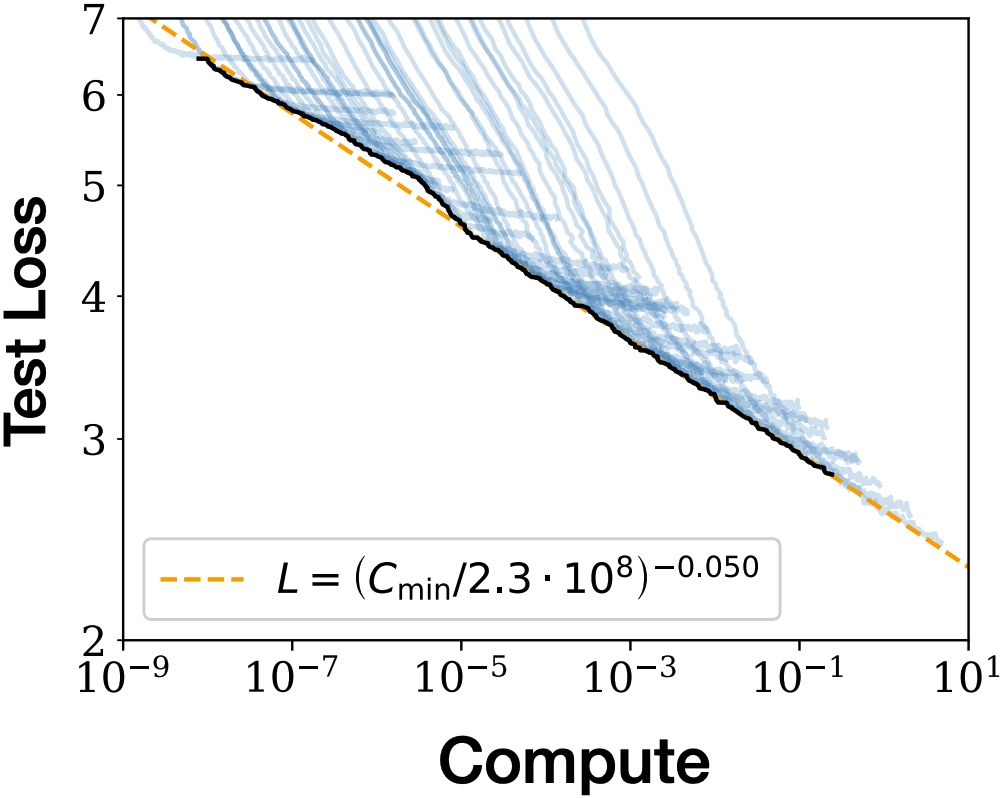
\includegraphics[height=0.7\textwidth]{screenshot/scaling_law.png} \\ 
\end{minipage}
}

\vspace{2.5mm}

\hrule


\visible<2->{

\vspace{1.5mm}

{\small

\textbf{Implication:} need to consider behavior of \textit{\color{NYUViolet}a sequence of progressively scaled-up runs}. 

}


\vspace{0.8mm}

\only<2>{
\begin{block}{Scale-aware Hyperparameters} \small
Let $n$ be the \textit{scaling dimension} (e.g., model width). The scaled HPs are defined as:
\[
    \cH_n({\color{FlatironOrange2}\vnu}, \vgamma) = ({\color{FlatironOrange2}\nu_1} n^{-\gamma_1}, \ldots, {\color{FlatironOrange2}\nu_{h}} n^{-\gamma_{h}}). 
\]
We refer to $\vnu = (\nu_1, \ldots, \nu_{h})$ as HPs (which are now \textit{scale-independent}).     
\end{block}
}

\visible<3->{

\begin{block}{Extrapolations from Small-scale Proxies}
\small
\centering
As the scale $n\to\infty$, if certain properties of interest (e.g., optimal hyperparameters) $(i)$ converge to a \textit{well-defined limit}, and $(ii)$ such convergence is \textit{``sufficiently fast''}, 
\colorbox{orange!12}{we can infer these properties of large models from small-scale proxies.}
\end{block}

}

}

\end{frame}  

\begin{frame}
\frametitle{Hyperparameter Tuning \& Transfer}
\vspace{1.5mm}


\parbox{0.5\linewidth}{ 

\vspace{-2mm}

\begin{minipage}[t]{0.96\linewidth} 
\begin{block}{}
\centering
\textbf{\color{FlatironOrange2!90!black}Tensor Program} {\small \color{lightgray!60!black}[Yang et al.~21,22]}. \\ Consider parameterizations that yield $(i)$ non-trivial (feature learning) limit, and $(ii)$ scale-independent HPs. 
\end{block}
\end{minipage}

\vspace{2mm}

{\small \color{lightgray!66!black}

\textit{Left:} standard param. ~
\textit{Right:} $\mu$ param. 

}

}
\parbox{0.49\linewidth}{
\begin{minipage}[t]{1\linewidth} 
\centering    
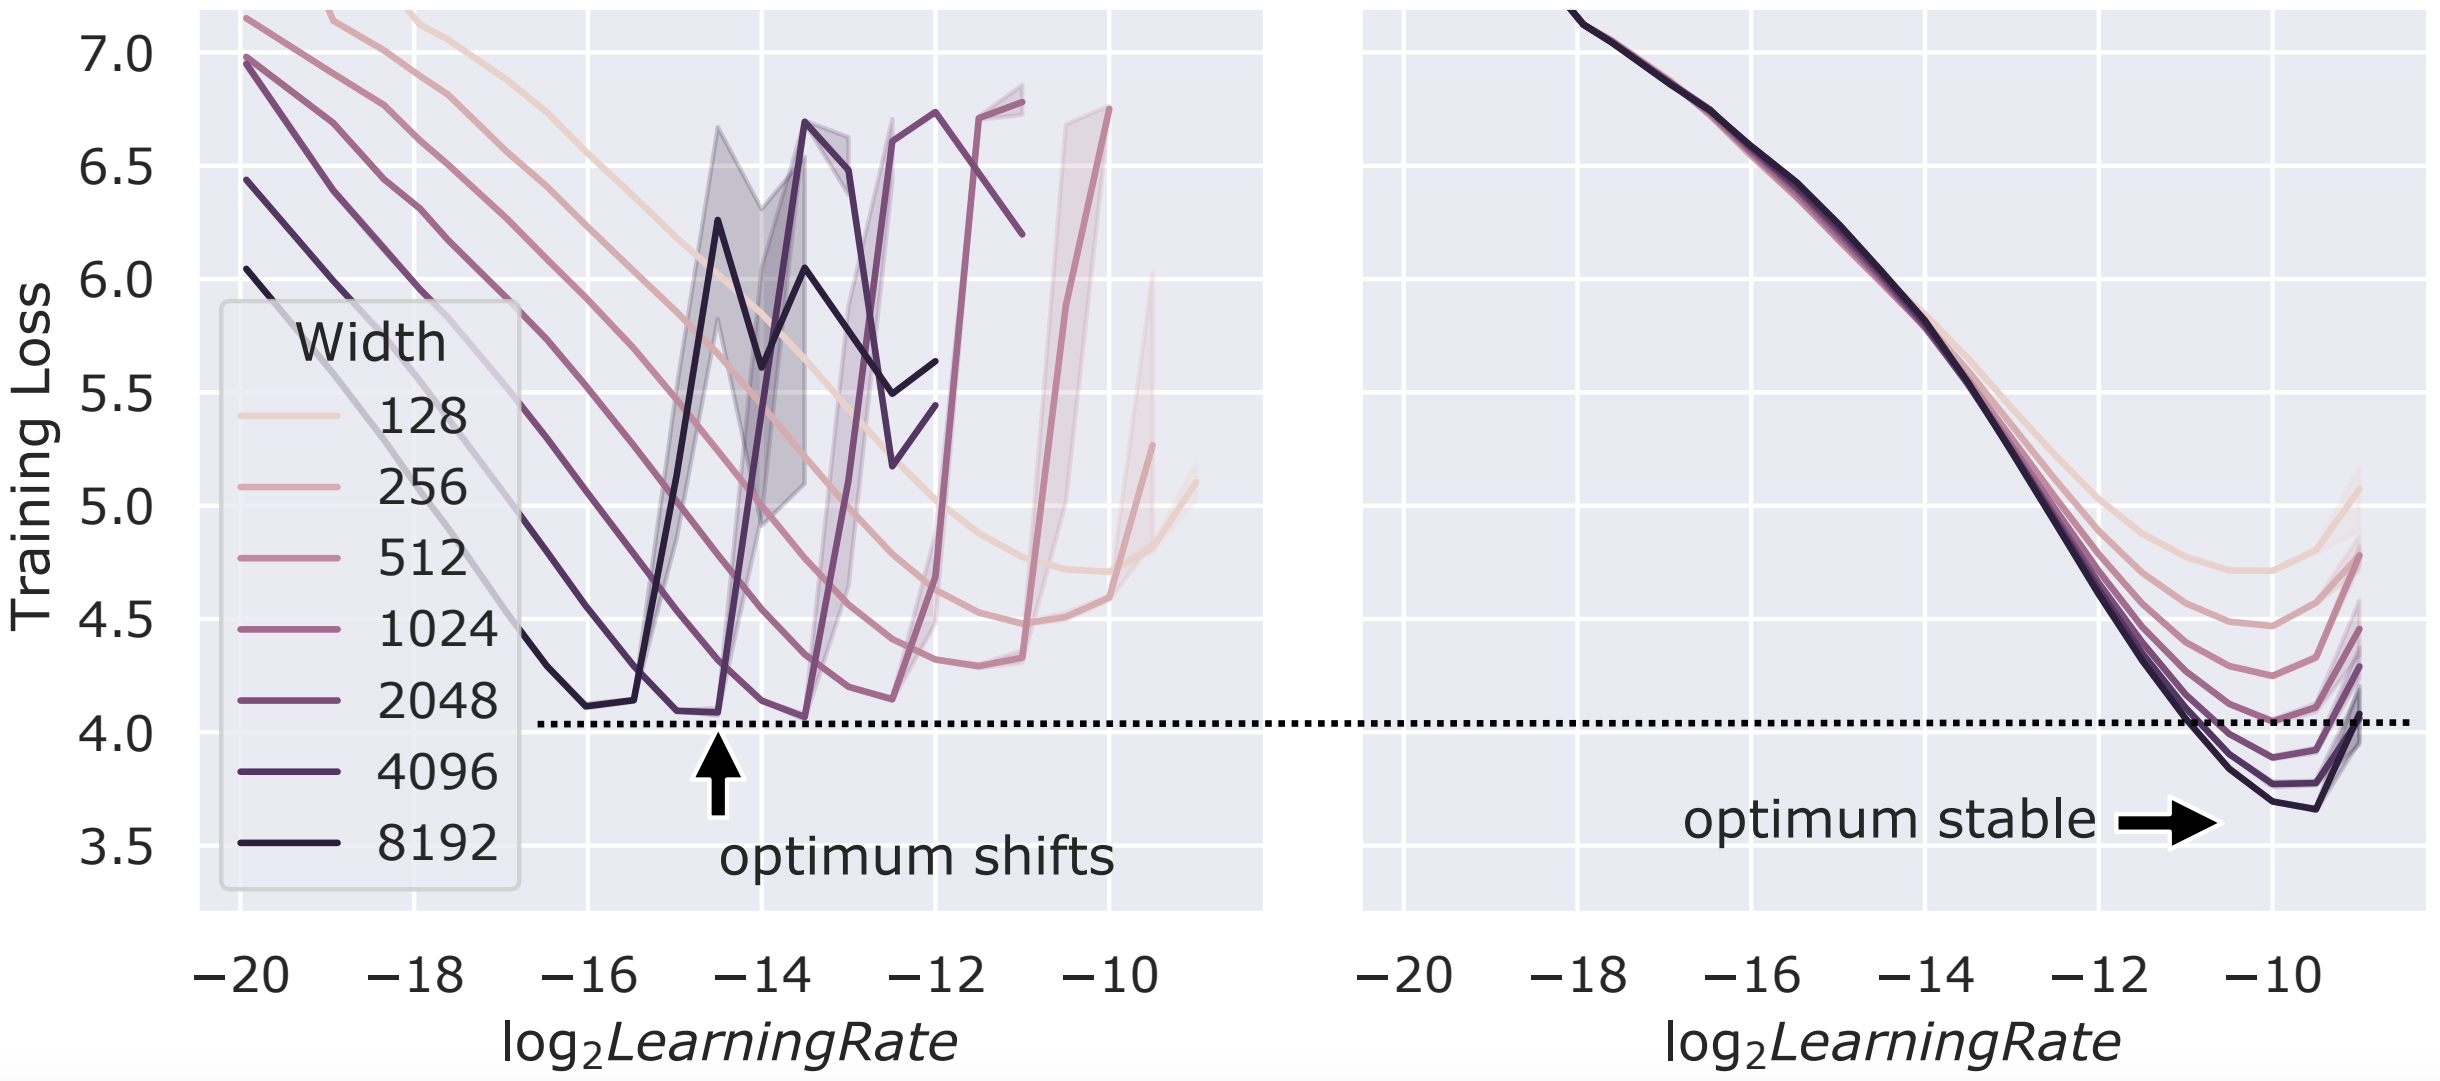
\includegraphics[height=0.48\textwidth]{screenshot/mu_transfer1.png} \\  
\end{minipage}
}

\visible<2->{

\vspace{3.mm}

\textbf{Benefit of HP stability:} Optimal HPs may be \textit{transferrable} across scale. 

\vspace{1.mm}

\parbox{0.32\linewidth}{ 


\begin{minipage}[t]{1\linewidth} 
\centering    
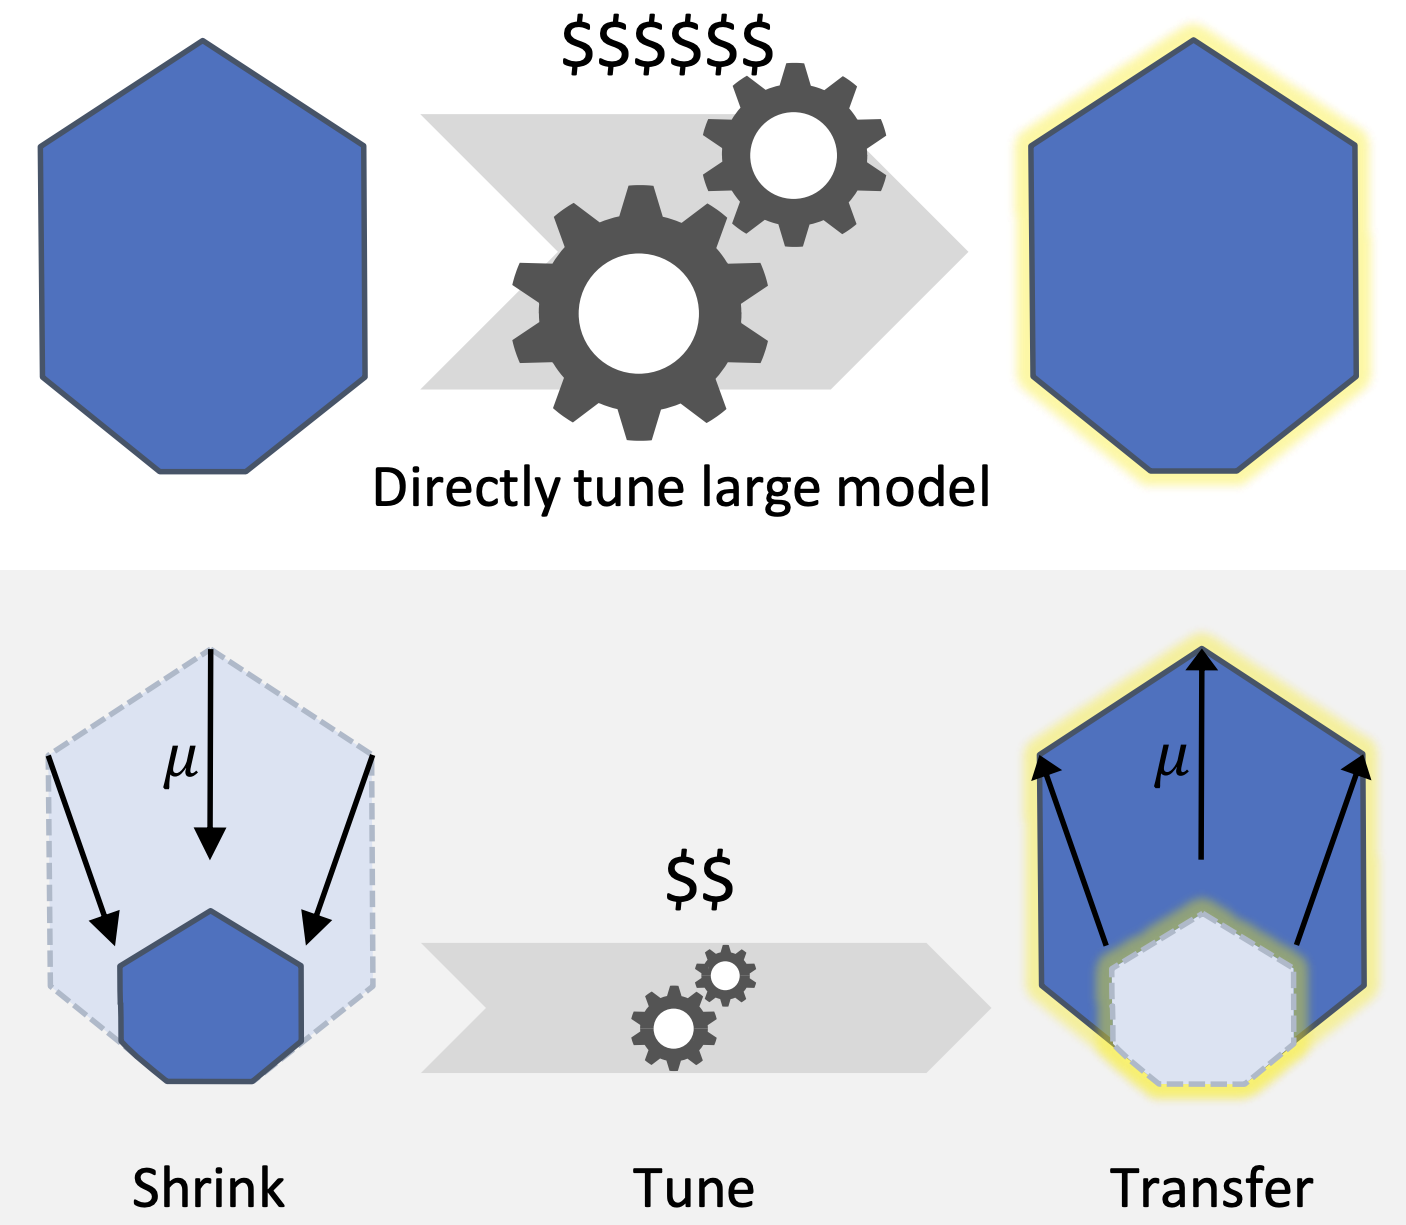
\includegraphics[height=0.86\textwidth]{screenshot/mu_transfer2.png} \\  
\end{minipage}

}
\parbox{0.67\linewidth}{
\begin{itemize}\setlength\itemsep{0.8em}
    \item \colorbox{red!12}{\textbf{Direct:}} sweep HPs on large models.  \\ \vspace{1mm}
    {\small \frownie\, \color{lightgray!60!black} Computationally prohibitive.}
    \pause\pause
    \item\colorbox{blue!12}{\textbf{Transfer:}} tune HPs on small models, and reuse optimal HPs on the large model. 
    \\ \vspace{1mm}
    {\small \color{lightgray!60!black} \textbf{Justification?} Requires optimal HPs to converge \textit{sufficiently fast} with respect to scale.}
\end{itemize}

}

 


}

\end{frame}  

\begin{frame}
\frametitle{Puzzle of Fast Hyperparameter Transfer}
\vspace{1.mm}

\textbf{Question:} when/why do optimal HPs converge sufficiently fast with scale?

\begin{itemize}\setlength\itemsep{0.15em}
    \item \colorbox{teal!12}{$\vnu^*_n$}: optimal {\color{FlatironOrange2!90!black}hyperparameter} (e.g., \textit{learning rate}) at scale $n$. 
    \item \colorbox{teal!12}{$\phi^*_n$}: optimal {\color{FlatironOrange2!90!black}performance} (e.g., \textit{validation loss}) at scale $n$. 
\end{itemize}

\vspace{0.5mm} 

\pause

\begin{alertblock}{}
\centering
Transfer is beneficial when $\vnu^*_n \to \vnu^*_\infty$ ``faster'' than $\phi^*_n \to \phi^*_\infty$.   
\end{alertblock}

\vspace{1mm}
\pause


\begin{columns}[T,onlytextwidth]
  % Left column
  \begin{column}{0.54\textwidth}
    % The sentence (appears from slide 3, sits at top because columns are top-aligned)
    \onslide<3->{\small 
      Scale-aware HPs (e.g., $\mu$P) yield well-defined $\vnu^*_\infty$ {\color{lightgray!66!black}(i.e., optima do not drift with scale)}, but do not entail \textit{stability \& fast convergence}.
    }

    \vspace{-3.75mm}

    % The block: reserve its height on all overlays, show from slide 5
    \visible<5->{%
      \small
      \begin{minipage}[t]{0.96\linewidth} \begin{block}{\small {\color{FlatironOrange2} This work:} quantifying HP transfer} \centering \begin{enumerate}\setlength\itemsep{0em} \item \textit{\color{NYUViolet}Formal framework} for HP convergence. 
      \item \textit{\color{NYUViolet}Toy examples} where transfer works/fails. 
      \item \textit{\color{NYUViolet}Conjecture} \& empirical evidence: fast HP transfer via \textit{\color{FlatironOrange2!88!black}loss decomposition}. \end{enumerate} \end{block} \end{minipage}
    }
  \end{column}

  % Right column
  \begin{column}{0.46\textwidth}
    \only<3|handout:0>{%
      \centering
      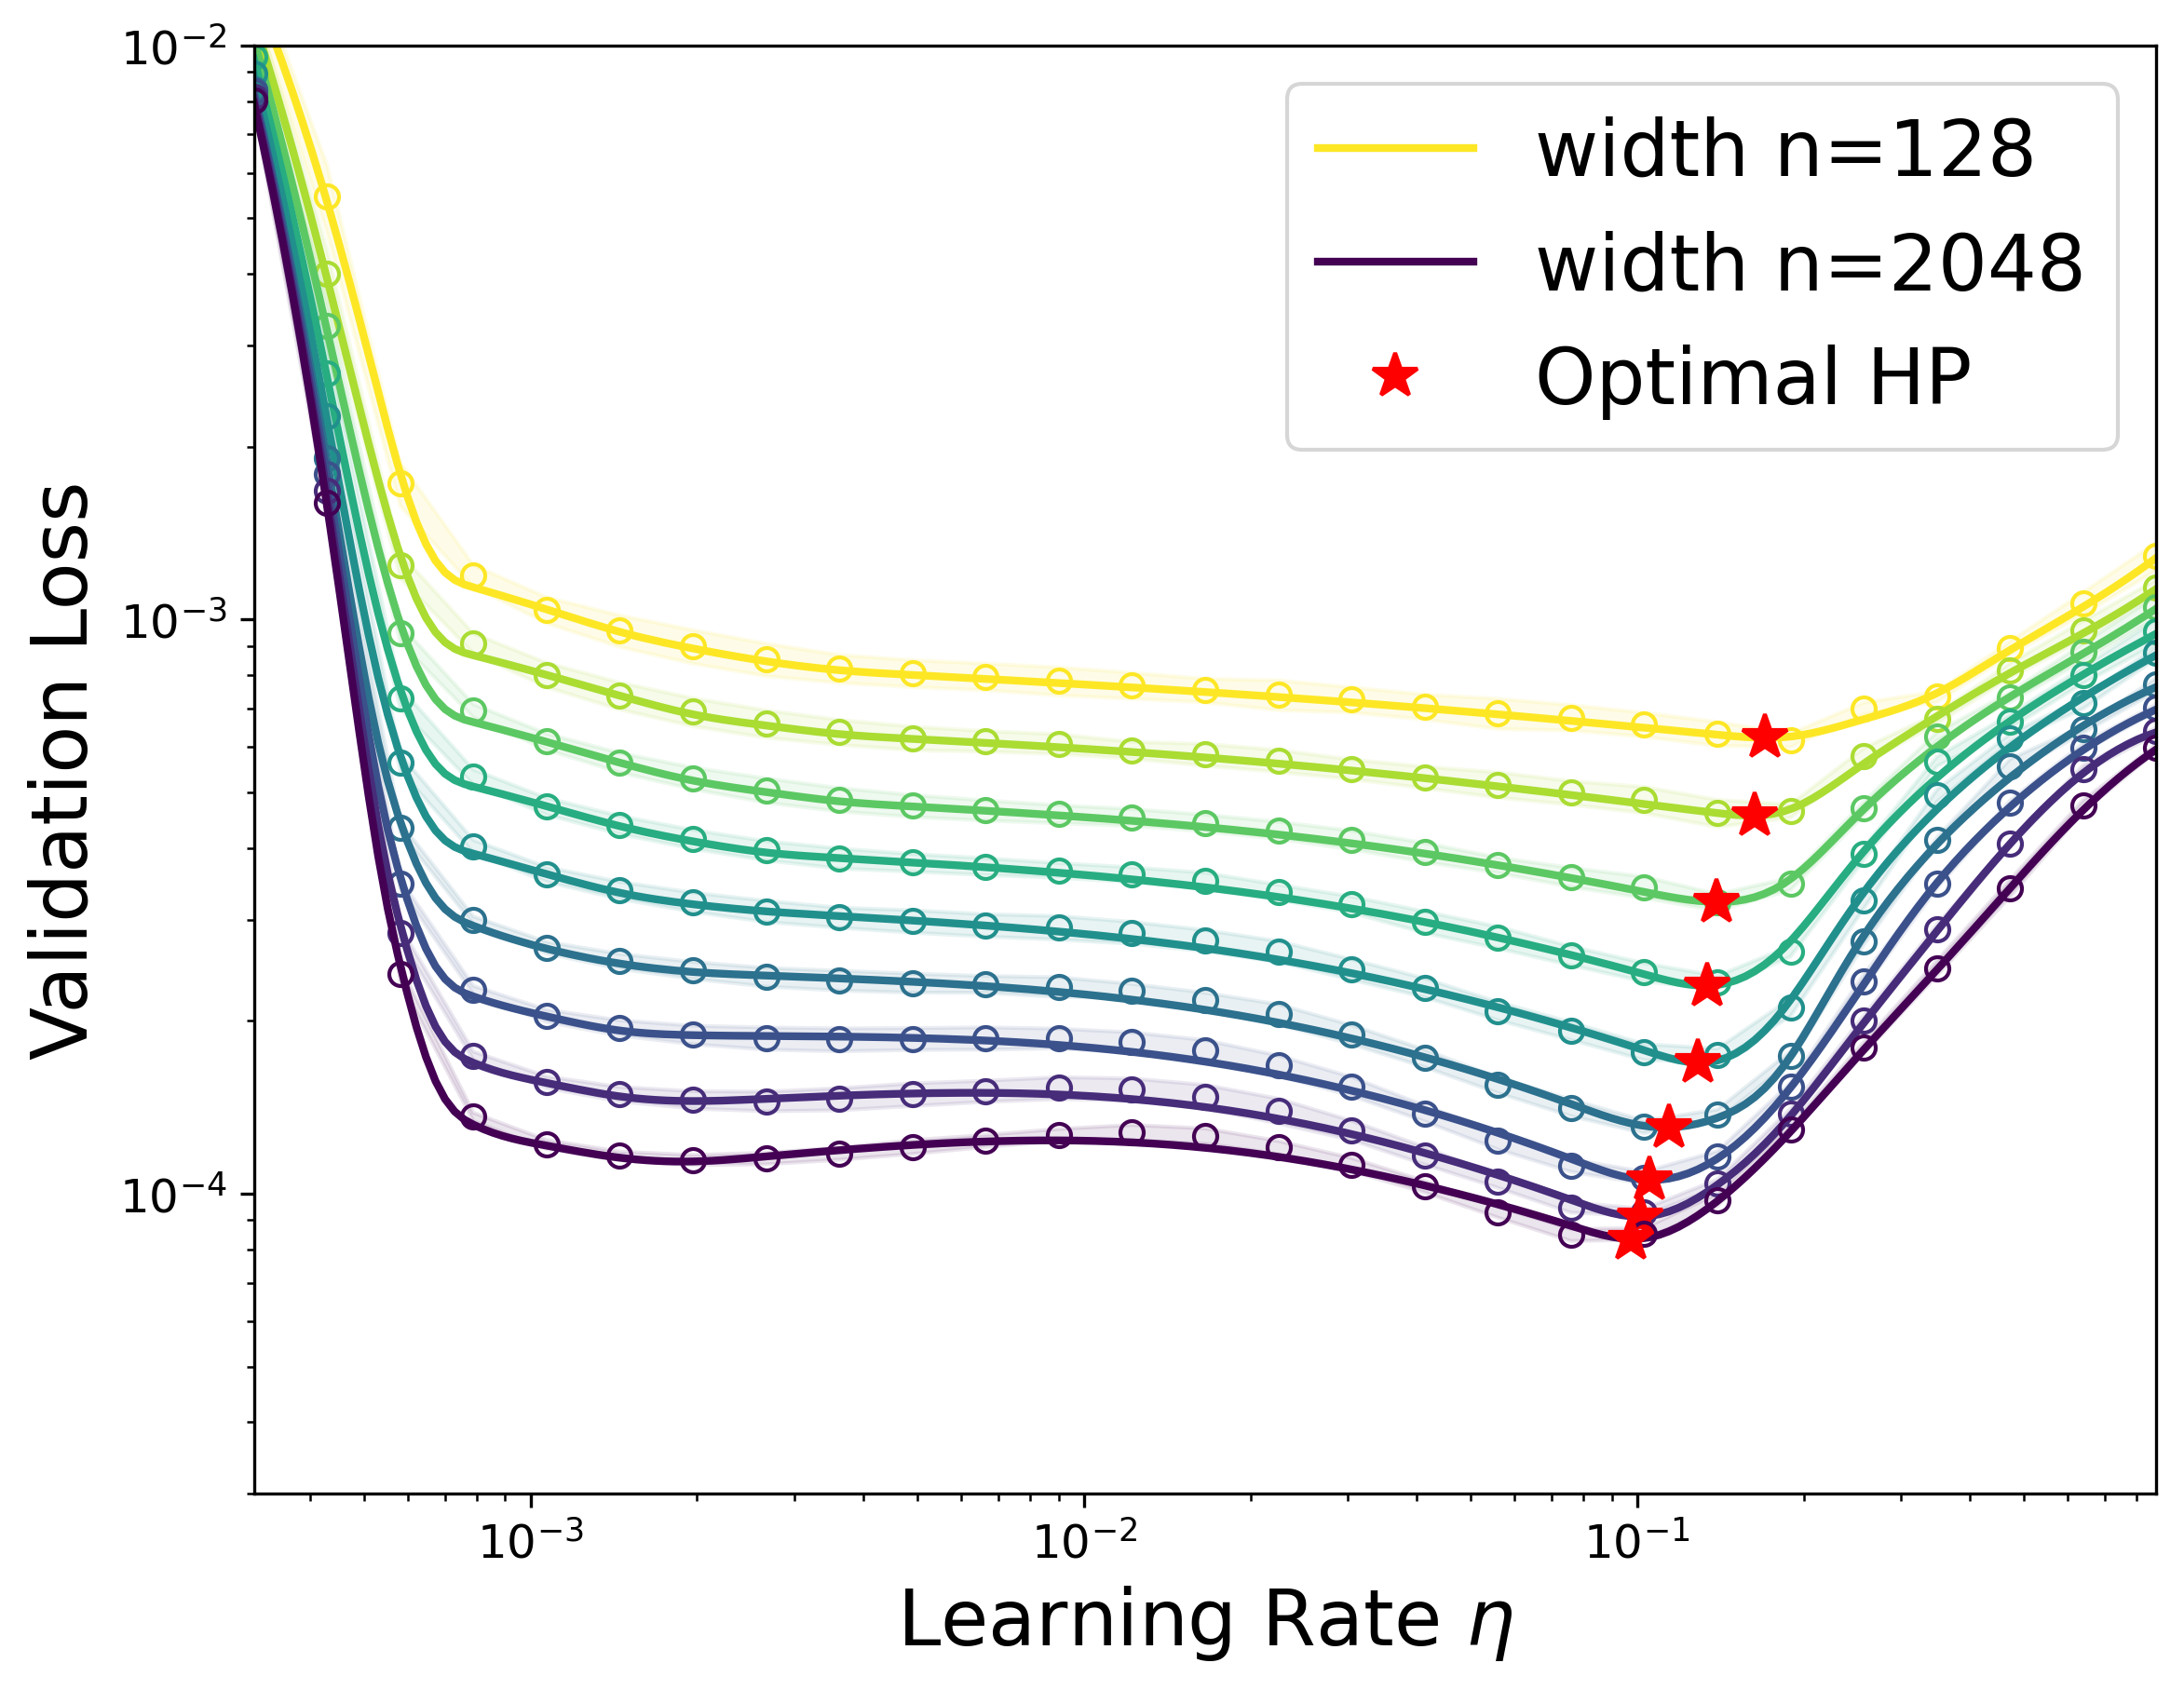
\includegraphics[width=\linewidth]{figure/two_layer_ReLU_k_16_d_64_regression_loss_early.png}
    }
    \only<4->{%
      \centering
      
\includegraphics[width=\linewidth]{figure/two_layer_ReLU_k_16_d_64_regression_loss.png}
    }
  \end{column}
\end{columns}


\end{frame}  


